\documentclass[a4paper,10pt]{article}
\usepackage[utf8]{inputenc}
\usepackage{graphicx}

%opening
\title{Projet Aspirateur v2}
\author{\texttt{Terral Naomie}\\
		\texttt{Rodriguez Charlotte}\\
		\texttt{Geshkovski Borjan}
		}
\date{06.02.2016}

\begin{document}

\maketitle

\begin{abstract}
Ceci est la deuxième version de notre projet Aspirator stochy debilum. Le code est organisé de manière modulaire. 
\end{abstract}

\section*{Organisation des données}
Pour lancer le programme il fauat exécuter le fichier launch.py. Le module fonctionnel (monde.py) se trouvent dans le dossier data.\\ 

\begin{center}
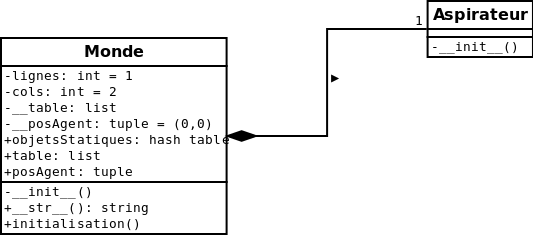
\includegraphics[scale=0.5]{architecture}
\end{center}


\begin{itemize}
 \item \texttt{objetsStatiques}: dictionnaire dont la clé est l'identifiant de l'élément contenu dans le monde. La clé fait référence à un tuple contenant la signification de l'élément et le caractère qu'on lui associe;
 \item \texttt{Monde()} : contient notre environnement. Nous allons décrire les différents attributs et méthodes:
  \begin{itemize}
  \item \texttt{\_\_init\_\_(aspirateur,lignes,colonnes)} : Constructeur de l'envrironnement;
  \item \texttt{objetsStatiques} : Renvoie objetsStatiques localement dans le monde;
  \item \texttt{table} : Renvoie l'état du monde;
  \item \texttt{posAgent} : Renvoie la position de l'aspirateur;
  \item \texttt{agent} : Renvoie l'agent (un aspirateur);
  \item \texttt{historique} : Renvoie l'ensemble d'etats; durant une simulation;
  \item \texttt{perfGlobale} : Renvoie la performance globale de l'aspirateur;
  \item \texttt{applyChoix(action)} : Change le monde en fonction d'une action choisie par l'aspirateur, et renvoie une evaluation de cette action; 
  \item \texttt{getPerception(capteurs)} : Renvoie le contenu dans les capteurs de l'aspirateur;
  \item \texttt{\_\_str\_\_} : Affichage du monde (état et aspirateur);
  \item \texttt{step} : Une etape pendant une simulation;
  \item \texttt{simulation(n)} : Simulateur d'un environnement de n etapes;
  \item \texttt{initialisation} : Initialise la position de l'aspirateur et l'état du monde de façon stochastique.
  \item \texttt{updateWorld}: MaJ du monde.
  \end{itemize}
 \item \texttt{Aspirateur()}
 \begin{itemize}
 \item \texttt{\_\_init\_\_(capteurs, actions)} : Constructeur d'aspirateur ; 
 \item \texttt{vivant} : Dead or alive.
 \item \texttt{capteurs} :  Les cases que l'aspirateur peut voir ;
 \item \texttt{actions} : Les actions que l'aspirateur peut executer ;
 \item \texttt{getDecision(content)} : L'aspirateur choisit quoi faire en fonction du contenu de la case ; 
 \item \texttt{getEvaluation()} : Feedback ; 
 \item \texttt{setReward(reward)} : Reward mechanism ; 
 \end{itemize}
 \item \texttt{AspiClairVoyant()} :
 \item \texttt{AspiVoyant()}
\end{itemize}

\end{document}
